\subsection{Thermal Camera}

\subsubsection{Fundamentals of Thermal Imaging}

Thermal imaging is a non-contact sensing technique that visualizes the heat emitted by objects in the form of infrared (IR) radiation. Unlike conventional cameras that rely on reflected visible light, thermal cameras detect naturally emitted radiation from all objects with temperatures above absolute zero\footnote{\label{thermography}\url{https://en.wikipedia.org/wiki/Thermography}}.

This emitted radiation follows the principles of blackbody radiation, where the intensity and spectral distribution of emitted energy depend on the surface temperature of the object. The infrared region spans wavelengths from approximately 0.7~\textmu m to 1000~\textmu m and is subdivided into bands including Near-Infrared (NIR), Short-Wave Infrared (SWIR), Mid-Wave Infrared (MWIR), Long-Wave Infrared (LWIR), and Far-Infrared (FIR). Different sub-bands serve different applications depending on their wavelength-dependent properties\textsuperscript{\ref{thermography}}.

A thermal camera detects this radiation using infrared-sensitive sensors and converts the signal into a digital thermogram. These thermograms display spatial temperature variations: warmer regions emit more radiation and appear brighter, while cooler areas emit less and appear darker\textsuperscript{\ref{thermography}}.

The observed thermal pattern is influenced by material-specific properties such as thermal conductivity, heat capacity, density, and surface roughness. These determine an object’s thermal inertia—its resistance to temperature change—and cause different materials to heat and cool at different rates~\cite{nikulin2018detection}. Techniques such as Differential Apparent Thermal Inertia (DATI) can leverage these thermal dynamics to enhance detection of buried objects like landmines.

Another critical factor is emissivity, which describes how effectively a surface emits thermal radiation. Emissivity values vary with material type, temperature, and wavelength, and must be considered in thermal imaging to ensure accurate temperature representation\textsuperscript{\ref{thermography}}.

Since different materials can have different thermal characteristics, i.e., thermal conductivity and heat capacity, a landmine can be thought of as an unnatural volume for flow of the heat inside the soil. This causes a specific spatiotemporal thermal pattern on the soil surface, which can be detected by IR imaging systems. 


\subsubsection{Camera Performance Parameters}

The performance of a thermal imaging system depends not only on the fundamental physics of infrared radiation but also on the specific characteristics of the camera. In the context of drone-based landmine detection, where targets are small, low-metal content objects with subtle thermal signatures, careful selection of the thermal camera's parameters is essential. Key factors include the spectral band, thermal sensitivity (NETD), pixel resolution, field of view (FOV), and ground sample distance (GSD). These parameters determine the camera’s ability to detect small temperature variations over a wide area, resolve details at high altitude, and distinguish buried landmines from their surrounding environment.


\paragraph{Spectral Band}
The infrared spectrum can be divided into five regions: NIR (0.7–1.4~\textmu m), SWIR (1.4–3~\textmu m), MWIR (3–8~\textmu m), LWIR (8–14~\textmu m), and FIR (15–1000~\textmu m). Among these, MWIR and LWIR are collectively known as the Thermal Infrared bands, which are used for passive thermal imaging due to their high atmospheric transmission and independence from external light sources. Unlike SWIR, which relies on reflected radiation, both MWIR and LWIR detect emitted heat and are effective under a wide range of environmental conditions\footnote{\label{LWIR}\url{https://www.shalomeo.com/LWIR-MWIR-Thermal-Imaging-Camera-shalomeo.html}}.

These thermal bands provide imaging based on temperature differences and are tolerant to obscurants like fog, smoke, and dust. They also function reliably regardless of visible lighting conditions, which is essential for buried landmine detection. According to Planck’s Law, thermal emission from objects increases with temperature, and the peak emission wavelength shifts inversely with temperature. As shown in Figure~\ref{fig:wien_law}, objects at ambient temperature (~300~K) emit radiation most strongly in the LWIR range (8–12~\textmu m). In contrast, only at high temperatures (~1000~K) does the emission peak shift into the MWIR range\textsuperscript{\ref{LWIR}}.

Atmospheric transmission also varies by wavelength. The regions with minimal atmospheric absorption—called atmospheric windows—determine which bands are suitable for long-range imaging. While MWIR has slightly lower absorption in humid or oceanic conditions, LWIR offers a broader and more stable atmospheric window, especially in the 8–12~\textmu m range, making it ideal for imaging terrestrial objects in standard environments\textsuperscript{\ref{LWIR}}. See Figure~\ref{fig:atmos_window}.

\begin{figure}[h!]
    \centering
    \begin{subfigure}[b]{0.48\linewidth}
        \centering
        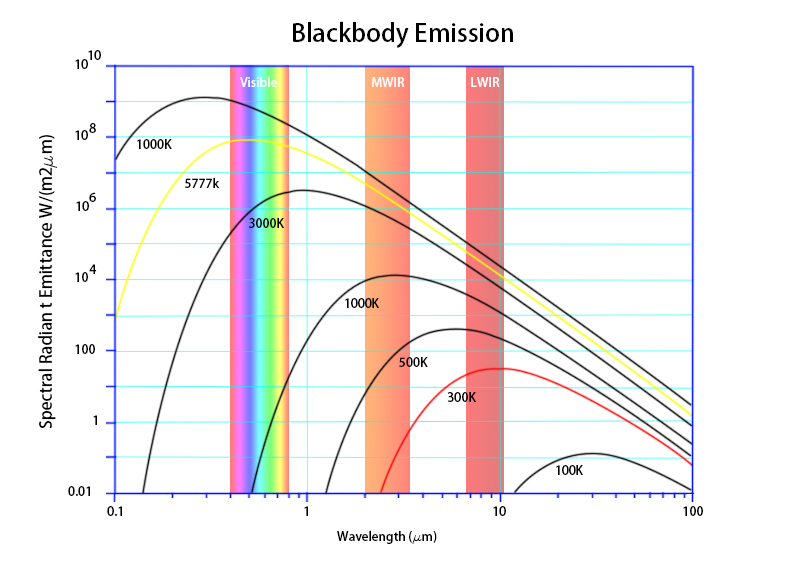
\includegraphics[height=3cm]{figs/Huirui/wien_law_plot.png}
        \caption{Planck spectral emission curve for different temperatures\textsuperscript{\ref{LWIR}}.}
        \label{fig:wien_law}
    \end{subfigure}
    \hfill
    \begin{subfigure}[b]{0.48\linewidth}
        \centering
        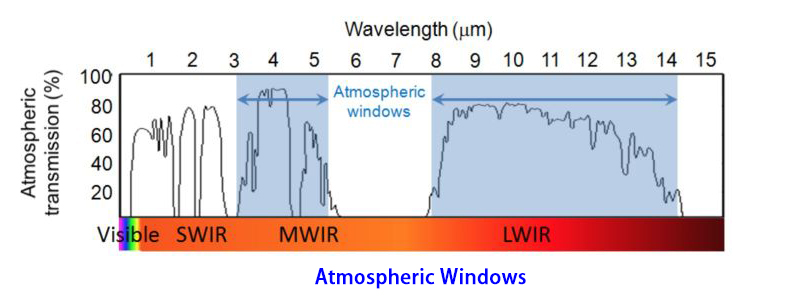
\includegraphics[height=3cm]{figs/Huirui/atmospheric_window_plot.png}
        \caption{Atmospheric transmission across infrared wavelengths\textsuperscript{\ref{LWIR}}.}
        \label{fig:atmos_window}
    \end{subfigure}
    \caption{Infrared sensing fundamentals.}
\end{figure}

The internal sensor type also varies by spectral band. MWIR cameras use cooled infrared detectors, which require cryogenic cooling to suppress their own thermal emissions. These systems operate by detecting individual high-energy photons using photodetectors in semiconductor materials. Although bulky and expensive, they offer excellent image quality, particularly for targets near or below room temperature. LWIR cameras typically use uncooled detectors, such as microbolometers, which sense changes in resistance, current, or voltage as they absorb infrared radiation. These sensors are smaller, more affordable, and energy-efficient, though they generally offer lower resolution and are more sensitive to their own heat signature\textsuperscript{\ref{thermography}}.

Given the need to detect subtle temperature variations in ambient conditions, coupled with the payload limitations of drone systems, LWIR is chosen as the preferred spectral band for our application.


\paragraph{Noise Equivalent Temperature Difference (NETD)}

NETD is defined as the smallest temperature difference that a thermal camera can detect, corresponding to a signal-to-noise ratio of 1. For instance, a camera with a NETD of 100~mK (0.1~\textdegree C) can theoretically distinguish a 25.1~\textdegree C drone against a 25.0~\textdegree C sky\footnote{\url{https://sierraolympia.com/what-is-netd-and-why-does-it-matter/}}. In practical terms, NETD determines the sensitivity of the sensor to small thermal contrasts between an object and its background, which is critical for identifying subtle temperature anomalies caused by buried landmines.

To estimate a suitable NETD threshold for our system, we refer to an experimental study where researchers applied infrared heating to sand containing buried landmines, then monitored the thermal signature as the surface cooled through natural convection—similar to conditions under solar heating~\cite{lamorski2002thermal}. Table~\ref{tab:netd_table} presents the maximum temperature differences observed using both thermocouples and thermal imaging at various depths and moisture levels.

It is important to note that the experimental heating used an infrared lamp, providing stronger and more concentrated energy than natural sunlight. In real-world scenarios, solar heating is more gradual and extends over longer periods, with additional influences from soil moisture and environmental variability. As a result, the values in Table~\ref{tab:netd_table} represent the upper bound of thermal contrast achievable under controlled conditions.

Considering these factors, we conservatively estimate that temperature differences of 0.5--1.0~\textdegree C are realistic in field conditions. To reliably detect such contrasts, a thermal camera with NETD ≤ 500~mK is recommended for this project.

\begin{table}[H]
    \centering
    \caption{Maximum temperature differences measured by both the thermocouples and the infrared camera and the duration of the cooling phase before they develop~\cite{lamorski2002thermal}.}
    \label{tab:netd_table}
    \scriptsize
    \begin{tabular}{ccccc}
        \toprule
        \textbf{Moisture content} & \textbf{Type of measurement} & \textbf{2 cm Depth} & \textbf{3 cm Depth} & \textbf{4 cm Depth} \\
        \midrule
        \multirow{2}{*}{Dry sand} 
            & Thermocouple & 1.3 °C, 20 min & 0.5 °C, 10 min & 1.5 °C, 10 min \\
            & IR Image     & 1.5 °C, 15 min & 1.0 °C, 30 min & Not observed \\
        \midrule
        \multirow{2}{*}{2.5\% water} 
            & Thermocouple & Not recorded   & 4.0 °C, 20 min & 1.2 °C, 15 min \\
            & IR Image     & 3.0 °C, 10 min & 3.5 °C, 10 min & 2.0 °C, 20 min \\
        \midrule
        \multirow{2}{*}{5\% water} 
            & Thermocouple & 2.4 °C, 10 min & 1.4 °C, 15 min & 2.0 °C, 20 min \\
            & IR Image     & 3.0 °C, 15 min & 3.0 °C, 15 min & 3.0 °C, 30 min \\
        \midrule
        \multirow{2}{*}{10\% water} 
            & Thermocouple & 3.8 °C, 10 min & 1.4 °C, 20 min & 1.1 °C, 10 min \\
            & IR Image     & 4.0 °C, 15 min & 1.8 °C, 30 min & 2.5 °C, 30 min \\
        \bottomrule
    \end{tabular}
\end{table}


\paragraph{Pixel Resolution}
Pixel resolution refers to the number of pixels in the thermal camera’s detector array and directly affects the level of detail the camera can capture. It is typically expressed as width × height, and common values resolutions include 160×120 (low), 320×240 (medium), and 640×480 (high). Higher resolution enables more precise thermal imaging and improved object discrimination, especially critical for small targets like buried landmines, but it also increases cost, power consumption, and weight\textsuperscript{\ref{thermography}}. 

Because our project involves thermal scanning from relatively high altitudes, we require a resolution that is as high as possible to preserve detail and accuracy across a wide field of view. At the same time, drone payload capacity and sensor cost must also be considered. Therefore, although some extremely high resolution cameras with 1280×1024 detectors exist, we select 640×480 as an optimal balance between image quality, affordability, and hardware feasibility.


\paragraph{Field of View (FOV) and Instantaneous Field of View (IFOV)}

The Field of View (FOV) of a thermal camera defines the total angular extent within which the camera can detect radiation. For drone-based applications where the thermal camera is mounted in a nadir (downward-facing) orientation, the FOV spans two angular directions—commonly referred to as the horizontal and vertical FOV. While these terms originate from camera sensor geometry, in this aerial imaging context, both angular fields lie in the horizontal plane relative to the ground. That is, the horizontal FOV corresponds to the width of the captured ground area, and the vertical FOV corresponds to the length of the coverage area.

The Instantaneous Field of View (IFOV), by contrast, refers to the angular field covered by a single pixel, and it determines the effective spatial resolution of the system.

Figure~\ref{fig:fov_ifov} illustrates the two-dimensional geometry of FOV and IFOV. In this case, the thermal sensor is assumed to be square-shaped, meaning its physical dimensions and pixel resolution are equal along both axes. As a result, the angular FOV and IFOV are also identical in both directions. This assumption simplifies the resolution and coverage calculations presented in the next sections, though in practice, FOV may differ between horizontal and vertical axes depending on sensor shape and lens design.

The angular field of view (FOV) and instantaneous field of view (IFOV) can be calculated as:

\begin{equation}
    FOV = 2 \cdot \tan^{-1} \left( \frac{a}{2f} \right)\footnote{\label{FOV}\url{https://hvoltbb.github.io/random/posts/fov.html}}
\end{equation}

\begin{equation}
    IFOV = 2 \cdot \tan^{-1} \left( \frac{\delta a}{2f} \right)\textsuperscript{\ref{FOV}}
\end{equation}

where \( f \) is the focal length of the lens, \( a \) is the physical width of the sensor, and \( \delta a \) is the width of a single pixel.

For a fixed flying height and pixel resolution, a wider FOV enables the drone to scan a larger ground area in a single frame, improving coverage efficiency. However, this increases the IFOV—each pixel covers a broader region—reducing spatial detail. Conversely, a narrower FOV improves detail by shrinking the IFOV, but at the cost of reduced area per scan. This trade-off is critical in drone-based landmine detection and must be considered when selecting lens focal length and flight altitude for our project.

\begin{figure}[H]
    \centering
    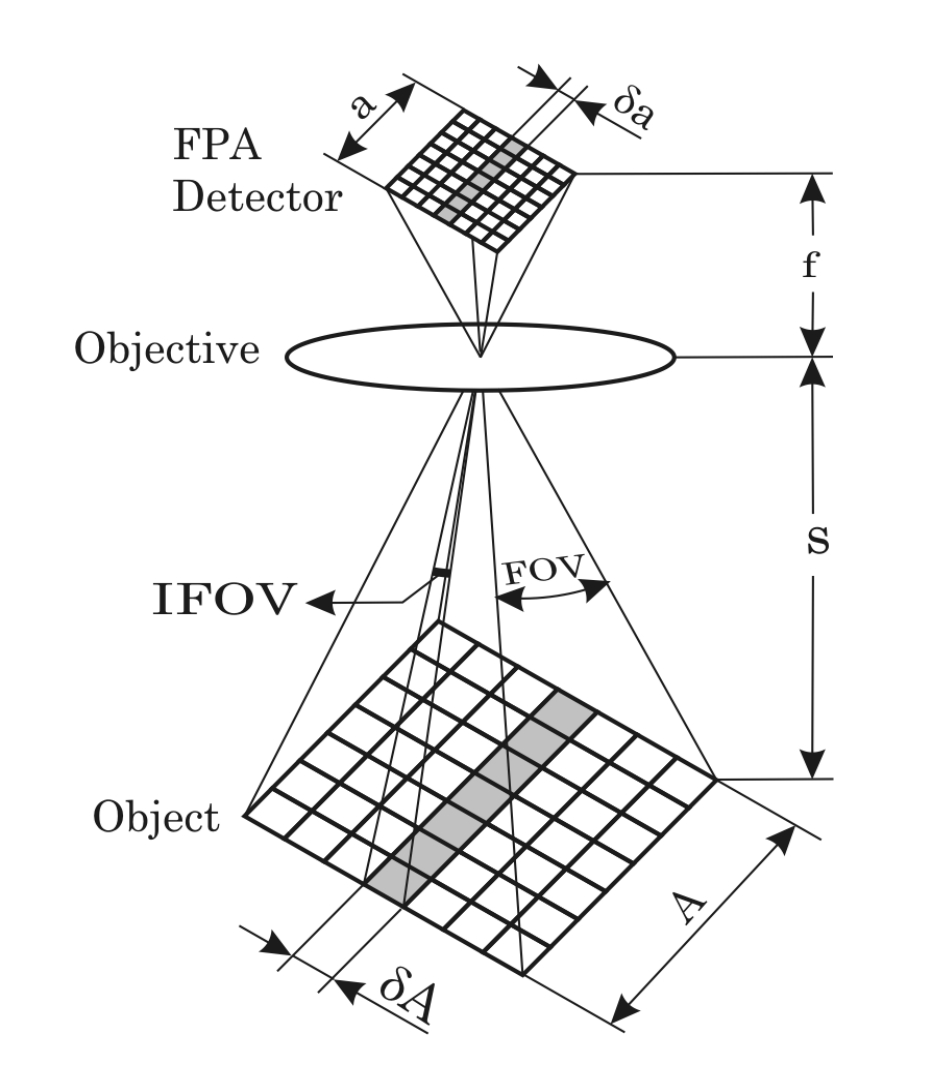
\includegraphics[width=0.3\textwidth]{figs/Huirui/fov_ifov_2d_diagram.png}
    \caption{FOV and IFOV for optical system~\cite{pencheva2006design}.}
    \label{fig:fov_ifov}
\end{figure}


\paragraph{Ground Sample Distance (GSD)}
GSD is the physical ground distance represented by one pixel in an image. For instance, a GSD of 1.4~cm/pixel means each pixel covers a 1.4~cm × 1.4~cm area on the ground\footnote{\url{https://en.wikipedia.org/wiki/Ground_sample_distance}}. GSD depends on drone height, FOV, and pixel resolution. Since anti-personnel landmines are typically ~6–10~cm in diameter, based on Table~\ref{tab:apm_specs}, we aim to have at least 5–6 pixels span the landmine footprint. Thus, we target a GSD of approximately 1.4~cm/pixel, which informs our choice of lens and flight altitude in later sections.


\subsubsection{Thermal Camera Selection}

Based on the theoretical principles and performance criteria established in the previous sections, the thermal camera used in our drone system must satisfy several key constraints. First, the spectral range must lie in the LWIR band, as this aligns with the peak thermal emission of terrestrial objects at ambient temperatures. Second, the NETD must be no greater than 500~mK to detect subtle contrasts between landmines and their surrounding soil. Third, the camera should offer a pixel resolution of at least 640×480 to ensure sufficient spatial detail for high-altitude scanning. Additionally, the lens focal length and field of view must be chosen to achieve a ground sample distance (GSD) of approximately 1.4~cm/pixel at operational flight altitudes between 5–10 meters. Lastly, the weight and cost must be suitable for drone integration, considering payload limitations and overall system budget.

Because a thermal camera's performance is tightly coupled with its image resolution at a given altitude, we choose to first fix the camera model and then determine the appropriate flight parameters—particularly the altitude—to achieve our target GSD. This approach ensures that the selected camera can realistically support the resolution requirements of the mission. The derivation of suitable drone height and corresponding coverage area will be addressed in the next section, once a viable thermal camera has been selected.

To identify candidate thermal cameras that meet these requirements, we reviewed a range of recent research papers (~\cite{baur2020applying,nikulin2018detection,krause2018diurnal,TENORIOTAMAYO2024105567,FORERORAMIREZ2022104307,rs15040967,dena2020image,Fardoulis2020PROOFHS,butt2024uav,AgrawalChung2024ComparingSL,Popov2022MethodFM,TENORIOTAMAYO2023109443}) on drone-based landmine detection. These studies report the use of various thermal imaging sensors in both experimental and field settings. From these papers, we compiled a shortlist of commercially available models, with key specifications drawn from product datasheets. Table~\ref{tab:camera_specs} summarizes these thermal cameras, including their pixel resolution, NETD, lens focal length and field of view, spectral band, weight, and price. These entries will inform the final selection of the sensor for our system.

From Table~\ref{tab:camera_specs}, four cameras meet the minimum resolution requirement of 640 × 512 pixels: FLIR Vue Pro, FLIR Duo Pro R, FLIR Tau 2, and DJI Zenmuse XT. All of these operate in the LWIR range (7.5–13.5~µm), and their weight falls within the estimated payload capacity of our drone system (around 3.6~kg, as discussed in the hardware section).

Among the candidates, all four options provide excellent sensitivity with NETD values below 50~mK, with FLIR Tau 2 offering the best sensitivity at <30~mK. In terms of weight, the FLIR Tau 2 is also the lightest at 72~g, followed by FLIR Vue Pro (92–113.4~g), DJI Zenmuse XT (270~g), and FLIR Duo Pro R (325–375~g). In terms of price, however, DJI Zenmuse XT is the most expensive at 9900~USD, while FLIR Vue Pro is the most affordable at 3895~USD.

When evaluating integration with our custom drone, the DJI Zenmuse XT—while technically viable—introduces significant challenges. Designed for DJI drones, it requires proprietary gimbal mounts, power supply connectors, and control via DJI-specific protocols. Adapting this to our custom quadcopter would require custom hardware and potentially reverse-engineering DJI’s interface—making it impractical for our development timeline and platform.

This leaves us with three practical options: FLIR Vue Pro, FLIR Duo Pro R, and FLIR Tau 2. All three are known to integrate well with our companion computers. They support control over PWM or serial interfaces, and thermal data can be streamed or logged in real-time via USB or analog video output. The Odroid XU4, used in our system, supports Python or C++ camera control scripts, real-time telemetry feedback, and onboard data logging—all of which make integration with these FLIR models efficient and flexible.

Between these three, the FLIR Duo Pro R is heavier and more expensive than FLIR Vue Pro, without offering significant performance benefits. The FLIR Tau 2 provides slightly better sensitivity and weight, but its higher cost (nearly double) cannot be justified given the modest difference in performance (NETD: 30~mK vs 50~mK). Therefore, we select the FLIR Vue Pro as the optimal thermal imaging solution for our project. It offers a good balance of resolution, weight, NETD, integration compatibility, and affordability, making it highly suitable for drone-based landmine detection.


\subsubsection{Flight Parameter and Focal Length Selection}

Once the thermal camera has been selected, the next step is to determine the appropriate flight parameters, including the operational altitude and the focal length (or FOV) of the lens. The FLIR Vue Pro camera offers multiple focal lengths (9~mm, 13~mm, and 19~mm), each producing a different FOV. A shorter focal length yields a wider FOV, enabling larger ground coverage per image but at the cost of lower spatial resolution. Conversely, a longer focal length provides narrower FOV, resulting in higher resolution but reduced coverage.

As previously established in the parameter section, the target Ground Sample Distance (GSD) is approximately 1.4~cm/pixel, which defines the physical ground spacing between adjacent pixels in the thermal image. Given that the pixel resolution of the FLIR Vue Pro is fixed at 640~×~512, and that the FOV varies with focal length, we can use trigonometric relationships to calculate the required flight altitude and image coverage for each lens configuration.


\begin{table}[H]
\centering
\caption{Comparison of thermal camera models used in previous studies and considered for selection.}
\label{tab:camera_specs}
\scriptsize
\begin{minipage}{\textwidth}
\begin{tabular}{|c|c|c|c|c|c|c|}
\hline
\textbf{Thermal Camera} & \textbf{Pixel Resolution} & \textbf{NETD (mK)} & \textbf{Lens \& FOV (H × V)} & \textbf{Spectral Range (\textmu m)} & \textbf{Weight (g)} & \textbf{Price} \\
\hline

\textbf{FLIR Vue Pro\footnote{\url{https://flir.netx.net/file/asset/10907/original/attachment}}} 
& 640 × 512 & < 50 & 
\begin{tabular}[c]{@{}c@{}}9 mm: 69° × 56° \\ 13 mm: 45° × 37° \\ 19 mm: 32° × 26° \end{tabular} 
& 7.5 – 13.5 (LWIR) & 92 – 113.4 & 3895 (USD)\footnote{\url{https://groupgets.com/products/flir-vue-pro}} \\
\hline

\multirow{2}{*}{\textbf{FLIR Duo Pro R\footnote{\url{https://flir.netx.net/file/asset/8136/original/attachment}}}} 
& 640 × 512 & < 50 & 
\begin{tabular}[c]{@{}c@{}}13 mm: 45° × 37° \\ 19 mm: 32° × 26° \\ 25 mm: 25° × 20° \end{tabular} 
& 7.5 – 13.5 (LWIR) & 325 – 375 & 6599 (USD)\footnote{\url{https://www.tequipment.net/FLIR/DUO-PRO-R-640-19mm-9Hz/UAVs-and-Drones/}} \\
\cline{2-7}
& 336 × 256 & < 50 & 
\begin{tabular}[c]{@{}c@{}}9 mm: 35° × 27° \\ 13 mm: 25° × 19° \\ 19 mm: 17° × 13° \end{tabular} 
& 7.5 – 13.5 (LWIR) & 325 & 4499 (USD)\footnote{\url{https://dronedoctorusa.com/products/flir-duo-pro-r-336-30hz-19mm-open-box}} \\
\hline

\textbf{FLIR One Pro\footnote{\url{https://flir.netx.net/file/asset/14770/original/attachment}}} & 160 × 120 & 70 & 50° × 43° & 8 – 14 (LWIR) & 36.5 & 349 (GBP)\footnote{\url{https://www.flir.co.uk/products/flir-one-pro/?model=435-0006-03&vertical=condition+monitoring&segment=solutions}} \\
\hline

\textbf{FLIR One Edge Pro\footnote{\url{https://flir.netx.net/file/asset/5631/original/attachment}}} & 160 × 120 & 70 & 54° × 42° & 8 – 14 (LWIR) & 153 & 435 (GBP)\footnote{\url{https://www.flir.co.uk/products/flir-one-edge-pro/}} \\
\hline

\textbf{FLIR Tau 2\footnote{\url{https://www.unmannedsystemstechnology.com/wp-content/uploads/2012/04/FLIR-Tau2-Brochure.pdf}}} 
& 640 × 512 & < 30 & 
\begin{tabular}[c]{@{}c@{}}7.5 mm: 90° × 69° \\ 9 mm: 69° × 56° \\ 13 mm: 45° × 37° \\ 19 mm: 32° × 26° \end{tabular} 
& 7.5 – 13.5 (LWIR) & 72 & 6813 (USD)\footnote{\url{https://www.thermalvideo.com/46640001x.htm}} \\
\hline

\multirow{2}{*}{\textbf{DJI Zenmuse XT\footnote{\url{https://www.dji.com/uk/zenmuse-xt/specs}}\footnote{\url{https://www.thedroneproshop.com/blogs/product-info/dji-zenmuse-xt-specifications}}}} 
& 640 × 512 & < 50 & 
\begin{tabular}[c]{@{}c@{}}7.5 mm: 90° × 68° \\ 9 mm: 69° × 56° \\ 13 mm: 45° × 37° \\ 19 mm: 32° × 26° \end{tabular} 
& 7.5 – 13.5 (LWIR) & 270 & 9900 (USD)\footnote{\url{https://1updrones.com/product/zenmuse-xt-2-640x512-13mm/}} \\
\cline{2-7}
& 336 × 256 & < 50 & 
\begin{tabular}[c]{@{}c@{}}6.8 mm: 49.1° × 37.4° \\ 9 mm: 35° × 27° \\ 13 mm: 25° × 19° \\ 19 mm: 17° × 13° \end{tabular} 
& 7.5 – 13.5 (LWIR) & 270 & 7999 (USD)\footnote{\url{https://www.bhphotovideo.com/c/product/1318086-REG/dji_cp_zm_000337_zenmuse_xt_336x256_6_8mm.html}} \\
\hline

\end{tabular}
\end{minipage}
\end{table}


The following equations are used to relate GSD to camera geometry and flight parameters. The first expression defines GSD based on flight height and FOV:

\begin{equation}
    GSD = \frac{2 \cdot (height \cdot \tan(\frac{FOV}{2}))}{pixel\ resolution}
\end{equation}

By rearranging this equation, we calculate the required flight height to achieve a specific GSD:

\begin{equation}
    height = \frac{GSD \cdot pixel\ resolution}{2 \cdot \tan(\frac{FOV}{2})}
\end{equation}

Once the altitude is known, the total width and height of the imaged ground area (coverage area) can be calculated as:

\begin{equation}
    \text{Ground Dimension} = 2 \cdot \text{height} \cdot 
    \tan\left(\frac{FOV_{h,v}}{2}\right)
\end{equation}

Using these equations, we evaluate each of the three available focal lengths for the FLIR Vue Pro. By holding GSD constant at 1.4~cm/pixel and comparing the resulting ground coverage areas, we can determine the most efficient focal length and corresponding flight altitude for thermal landmine detection. The results are summarized in Table~\ref{tab:fov_results}. 

Interestingly, the ground coverage areas across all focal lengths are relatively similar, ranging between 62–65~m\textsuperscript{2}. However, the required flight height increases substantially with focal length—from 6.52~m at 9~mm to 15.62~m at 19~mm. Since the radiative flux received by the thermal sensor diminishes with increasing distance from the heat source (due to geometric spreading and atmospheric attenuation), a lower operating altitude reduces energy loss and maximizes signal strength. Therefore, the 9~mm focal length with its lower flight height of around 6~m is selected for this project as the optimal balance of resolution, coverage, and thermal signal fidelity.

\begin{table}[H]
\centering
\caption{Estimated Flight Height and Coverage Area for Different Focal Lengths (at GSD = 1.4~cm/pixel)}
\label{tab:fov_results}
\begin{tabular}{|c|c|c|c|}
\hline
\textbf{Focal Length (mm)} & \textbf{FOV (H × V)} & \textbf{Height (m)} & \textbf{Coverage Area (m\textsuperscript{2})} \\
\hline
9  & 69° × 56° & 6.52   & 62.09  \\
\hline
13 & 45° × 37° & 10.82  & 64.84  \\
\hline
19 & 32° × 26° & 15.62  & 64.63  \\
\hline
\end{tabular}
\end{table}
